% Packages

\documentclass[
	11pt, % Set the default font size, options include: 8pt, 9pt, 10pt, 11pt, 12pt, 14pt, 17pt, 20pt
	%t, % Uncomment to vertically align all slide content to the top of the slide, rather than the default centered
	%aspectratio=169, % Uncomment to set the aspect ratio to a 16:9 ratio which matches the aspect ratio of 1080p and 4K screens and projectors
]{beamer}
\setcounter{tocdepth}{1}
\usepackage{graphicx}
\usepackage[export]{adjustbox}
\graphicspath{{Images/}{./}} % Specifies where to look for included images (trailing slash required)
\usepackage{tikz}
\newenvironment{amatrix}[1]{
    \left[\begin{array}{@{}*{#1}{c}|c@{}}
}{%
    \end{array}\right]
}

\usepackage{booktabs} % Allows the use of \toprule, \midrule and \bottomrule for better rules in tables
\usepackage{pgfplots}
\usepackage{tikz}
\pgfplotsset{width=6cm, compat=newest, every tick label/.append style={scale=0.5}}
\usepackage{amsmath}
\usepackage{blkarray}% http://ctan.org/pkg/blkarray
\newcommand{\matindex}[1]{\mbox{\scriptsize#1}}% Matrix index

% Theme
\usetheme{Madrid}

% Font
\usefonttheme{serif}
\usepackage{newtxtext,newtxmath}
\usepackage[default]{lato}

% Inner theme
\useinnertheme{circles}

% Information
\title{Combinatorics}
\author{Kin Hei Wong}
\date{\today}
%%%%%%%%%%%%%%%%%%%%%%%%%%%%%%%%%%%%%%%%%%%%%%%%%%%%%%%%%%
\begin{document}

% Title slide
\begin{frame}
    \titlepage
\end{frame}

% Table of Content
\begin{frame}
    \frametitle{Presentation overview}
    \tableofcontents
\end{frame}
%%%%%%%%%%%%%%%%%%%%%%%%%%%%%%%%%%%%%%%%%%%%%%%%%%%%%%%%%%%
% Body slides

\section{9A: Basic counting methods}
\begin{frame}
    \frametitle{9A}
    \begin{center}
        \title{Basic counting methods}
        \maketitle
    \end{center}
\end{frame}

\begin{frame}[t]
    \frametitle{Basic counting methods}
    Tree diagram:
    \begin{block}{Example 1}
        A restaurant has a fixed menu, offering a choice of fish or beef for the main meal, and cake, pudding or ice-cream for dessert. How many different meals can be chosen?
    \end{block}
\end{frame}

\begin{frame}[t]
    \frametitle{Multiplication principle}
    \begin{block}{Multipliation principle}
        If there are $m$ ways of performing one task and then there are $n$ ways of performing
        another task, then there are $m\times n$ ways of performing both tasks.
    \end{block}
    \begin{block}{Example 2}
        Sandra has three different skirts, four different tops and five different pairs of shoes. How
        many choices does she have for a complete outfit?
    \end{block}
    \begin{block}{Example 3}
        How many paths are there from point P to R travelling from left to right? [This is also Graph Theory]\\
        \begin{center}
            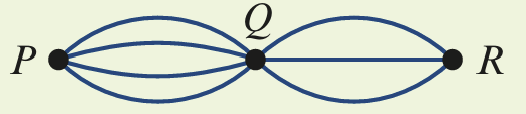
\includegraphics[width = 5cm]{Example3.png}
        \end{center}
    \end{block}
\end{frame}

\begin{frame}[t]
    \frametitle{Addition principle}
    \begin{block}{Addition principle}
        Suppose there are $m$ ways of performing one task and $n$ ways of performing another task. 
        If we cannot perform both tasks, then there are $m+n$ ways to perform one of the tasks.
    \end{block}
    \begin{block}{Example 4}
        To travel from Melbourne to Sydney tomorrow, Kara has a choice between three different flights 
        and two different trains. How many choices does she have?
    \end{block}
    \begin{block}{Example 5}
        How many paths are there from point A to E travelling from left to right?\\
        \begin{center}
            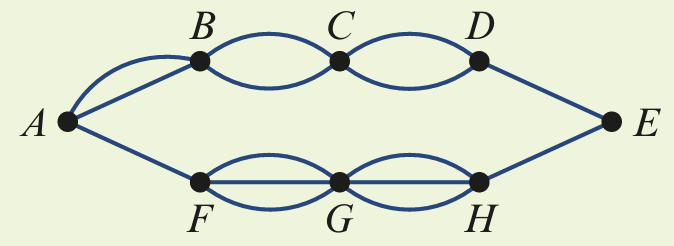
\includegraphics[width = 3cm]{Example5.png}
        \end{center}
    \end{block}
\end{frame}

\begin{frame}[t]
    \frametitle{Harder problems involving tree digram}
    \begin{block}{Example 6}
        A bag contains one blue token, two red tokens and one green token. Three tokens are removed from the bag and placed 
        in a row. How many arrangements are possible?
    \end{block}
\end{frame}

\begin{frame}
    \frametitle{Exercise 9A}
\end{frame}

%%%%%%%%%%%%%%%%%%%%%%%%%%%%%%%%%%%%%%%%%%%%%%%%%%%%%%%%%%%%%%%%%%%%%%%%%%%%%%%%%%%%%%%%%

\section{9B: Factorial notation and permutations}
\begin{frame}
    \frametitle{9B}
    \begin{center}
        \title{Factorial notation and permutations}
        \maketitle
    \end{center}
\end{frame}

\begin{frame}
    \frametitle{Factorial notation}
    $n! = n \cdot (n-1) \cdot (n-2) \cdot \dots 2 \cdot 1$\\
    $n! = n \cdot (n-1)!$
    \begin{block}{Example 7}
        \begin{enumerate}
            \item $3!$
            \item $\frac{50!}{49!}$
            \item $\frac{10!}{2!8!}$
        \end{enumerate}
    \end{block}
\end{frame}

\begin{frame}[t]
    \frametitle{Permutations}
    Permutation: ordered arrangments of a collections of objects
    \begin{block}{Example 8}
        Using a tree diagram, list all the permutations of the letters in the word CAT.
    \end{block}
    \begin{block}{Example 9}
        How many ways can six different books be arranged on a shelf?
    \end{block}
\end{frame}

\begin{frame}[t]
    \frametitle{More examples}
    \begin{block}{Example 11}
        How many four-digit numbers can be formed using the digits 1,2,3 and 4 if:
        \begin{enumerate}
            \item they cannot be repeated
            \item they can be repeated?
        \end{enumerate}
    \end{block}
\end{frame}

\begin{frame}[t]
    \frametitle{Number of permutations}
    \begin{block}{Number of permutations}
        The number of permutations of $n$ objects taken $r$ at a time is denoted by the formula:\\
        $^nP_r = \frac{n!}{(n-r)!}$
    \end{block}
    Proof:
\end{frame}

\begin{frame}[t]
    \frametitle{Number of permutations}
    \begin{block}{Example 12}
        \begin{enumerate}
            \item Using the letters A,B,C,D and E without repetition, how many different two-letter arrangments are three?
            \item Six runners compete in a race. In how many ways can the gold, silver and bronze medals be awarded?
        \end{enumerate}        
    \end{block}
    \begin{block}{Example 13}
        How many ways can seven friends sit along a park bench with space for only four people?
    \end{block}
\end{frame}

\begin{frame}
    \frametitle{Exercise 9B}
\end{frame}

%%%%%%%%%%%%%%%%%%%%%%%%%%%%%%%%%%%%%%%%%%%%%%%%%%%%%%%%%%%%%%%%%%%%%%%%%%%%%%%%%%%%%%%%%

\section{9C: Permutations with restriction}
\begin{frame}
    \frametitle{9C}
    \begin{center}
        \title{Permutations with restriction}
        \maketitle
    \end{center}
\end{frame}

\begin{frame}[t]
    \frametitle{Restrictions}
    When considering permutations with restrictions, we deal with the restrictions first.
    \begin{block}{Example 14}
        \begin{enumerate}
            \item How many arrangements of the word DARWIN begin and end with a vowel?
            \item Using the digits 0,1,2,3,4 and 5 without repetition, how many odd four-digit numbers can you form?
        \end{enumerate}
    \end{block}
\end{frame}

\begin{frame}[t]
    \frametitle{Permutations with items grouped together}
    \begin{block}{Example 15}
        \begin{enumerate}
            \item How many arrangements of the word EQUALS are there if the vowels are kept together?
            \item How many ways can two chemistry, four physics and five biology books be arranged on a shelf if 
            the books of each subject are kept together?
        \end{enumerate}        
    \end{block}
\end{frame}

\begin{frame}
    \frametitle{Exercise 9C}
\end{frame}

%%%%%%%%%%%%%%%%%%%%%%%%%%%%%%%%%%%%%%%%%%%%%%%%%%%%%%%%%%%%%%%%%%%%%%%%%%%%%%%%%%%%%%%%%

\section{9D: Permutations of like objects}
\begin{frame}
    \frametitle{9C}
    \begin{center}
        \title{Permutations of like objects}
        \maketitle
    \end{center}
\end{frame}

\begin{frame}
    \frametitle{Permutations of like objects}
    \begin{block}{Permutations of like objects}
        The number of permutations of $n$ objects of which $n_1$ are alike, $n_2$ are alike, $\dots$ and $n_r$ are alike 
        is given by:\\
        $\frac{n!}{n_1!n_2!\dots n_r!}$
    \end{block}
    E.g.: WOOLLOOMOOLOO
\end{frame}

\begin{frame}[t]
    \frametitle{Example}
    \begin{block}{Example 16}
        \begin{enumerate}
            \item Find the number of permutations of the letters in the word RIFFRAFF.
            \item There are four identical knives, three identical forks and two identical spoons in a drawer. 
            They are taken out of the drawer and lined up in a row. How many ways can this be done?
        \end{enumerate}
    \end{block}
    \begin{block}{Example 17}
        This grid shown consist of unit squares. By travelling only right (R) or down (D) along the grid lines, how many paths 
        are there point A to point B?
        \begin{center}
            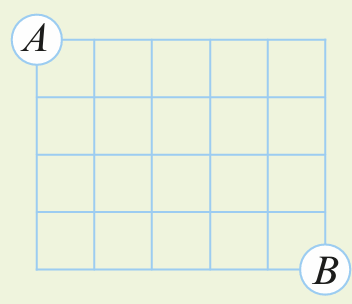
\includegraphics[width=2cm]{Example17.png}
        \end{center}
    \end{block}
\end{frame}

\begin{frame}
    \frametitle{Exercise 9D}
\end{frame}

%%%%%%%%%%%%%%%%%%%%%%%%%%%%%%%%%%%%%%%%%%%%%%%%%%%%%%%%%%%%%%%%%%%%%%%%%%%%%%%%%%%%%%%%%

\section{9E: Combinations}
\begin{frame}
    \frametitle{9C}
    \begin{center}
        \title{Combinations}
        \maketitle
    \end{center}
\end{frame}

\begin{frame}[t]
    \frametitle{Combinations}
    Combination($^nC_r$): a selection made regardless of order
    \begin{block}{Number of combinations}
        The number of combinations of $n$ objects taken $r$ at a time is given by the formula:\\
        $^nC_r = \frac{n!}{r!(n-r)!}$        
    \end{block}
    \begin{block}{Example 18}
        How many ways can two letters be chosen from the set{A,B,C,D}?
    \end{block}
    \begin{block}{Example 19}
        \begin{enumerate}
            \item A pizza can have three toppings chosen from nine options. How many different pizzas can be made?
            \item How many subsets of ${1,2,3,\dots,20}$ have exactly two elements?
        \end{enumerate}
    \end{block}
\end{frame}
\begin{frame}
\end{frame}

\begin{frame}[t]
    \frametitle{Examples}
    \begin{block}{Example 21}
        Consider a group of six students. In how many ways can a group of:\\
        \begin{enumerate}
            \item two student be selected
            \item four students be selected?
        \end{enumerate}
    \end{block}
\end{frame}

\begin{frame}[t]
    \frametitle{More examples}
    \begin{block}{Example 22}
        \begin{enumerate}
            \item Six points lie on a circle. How many triangles can you make using these points as the vertices?
            \item Each of the 20 people at a party shakes hands with every other person. How many handshakes take places?
        \end{enumerate}
    \end{block}
\end{frame}

\begin{frame}[t]
    \frametitle{More and more examples}
    \begin{block}{Example 23}
        From example 17's grid. By only travelling in right (R) and down (D) along the grid lines, how many paths are 
        there from point A to point B?
    \end{block}
\end{frame}

\begin{frame}
    \frametitle{Exercise 9E}
\end{frame}

%%%%%%%%%%%%%%%%%%%%%%%%%%%%%%%%%%%%%%%%%%%%%%%%%%%%%%%%%%%%%%%%%%%%%%%%%%%%%%%%%%%%%%%%%

\section{9F: Combinations with restriction}
\begin{frame}
    \frametitle{9F}
    \begin{center}
        \title{Combinations with restriction}
        \maketitle
    \end{center}
\end{frame}

\begin{frame}[t]
    \frametitle{Straight to examples}
    \begin{block}{Example 24}
        \begin{enumerate}
            \item Grace belongs to a group of eight workers. How many ways can a team of four workers be selected if Grace 
            must be on the team?
            \item A hand of card consists of five cards drawn from a deck of 52 playing cards. How many hand contain both 
            the queen and the king of hearts?
        \end{enumerate}
    \end{block}
    \begin{block}{Example 25}
        Four students are to be chosen from a group of eight students for the school tennis team. Two members of the group, Same 
        and Tess, do not get along and cannot both be on the team. How many ways can the team be selected?
    \end{block}
\end{frame}

\begin{frame}[t]
    \frametitle{Examples... examples... too many...}
    From seven women and four men in a workplace, how many groups of five can be chosen:\\
    \begin{enumerate}
        \item without restriction
        \item containing three women and two men
        \item containing at least one many
        \item containing at most one man?
    \end{enumerate}
\end{frame}

\begin{frame}[t]
    \frametitle{FUSION!}
    \begin{block}{Example 27}
        \begin{enumerate}
            \item How many arrangments of the letters in the word DUPLICATE can be made that have two vowels and three consonants?
            \item A president, vice-president, secretary and treasurer are to be chosen from a group containing 
            seven women and six men. How many ways can this be done if exactly two women are chosen?
        \end{enumerate}        
    \end{block}
\end{frame}

\begin{frame}
    \frametitle{Exercise 9E}
\end{frame}

%%%%%%%%%%%%%%%%%%%%%%%%%%%%%%%%%%%%%%%%%%%%%%%%%%%%%%%%%%%%%%%%%%%%%%%%%%%%%%%%%%%%%%%%%

\section{9G: Pascal's triangle}
\begin{frame}
    \frametitle{9G}
    \begin{center}
        \title{Pascal's triangle}
        \maketitle
    \end{center}
\end{frame}

\begin{frame}
    \frametitle{Pascal triangle}
\end{frame}

\begin{frame}
    \frametitle{Pascal's rule}
    $^nC_r = ^{n-1}C_{r-1} + ^{n-1}C_{r}, \text{where } 1\leq r<n$
    \begin{block}{Example 28}
        Given that $^{17}C_2$ = 136 and $^{17}C_3 = 680$, evaluate $^{18}C_3$.
    \end{block}
    \begin{block}{Example 29}
        Write down the $n=6$ row of Pascal's triangle and then write down the value of $^6C_3$.        
    \end{block}
\end{frame}

\begin{frame}[t]
    \frametitle{Subsets of a set}
    \begin{enumerate}
        \item The sum of the entries in row $n$ of Pascal's triangle is $2^n$. That is\\
        $^nC_0 + ^nC_1 + ^nC_2 + \dots + ^nC_n-1 + ^nC_n = 2^n$
        \item A set of size $n$ has $2^n$ subsets, including the empty set and the set itself.
    \end{enumerate}
    \begin{block}{Example 30}
        \begin{enumerate}
            \item Your friend offers you any of six books that she no longer wants. How many selectiosn are possible assuming that you take at least one book?
            \item How many subsets of ${1,2,3, \dots, 10}$ have at least two elements?
        \end{enumerate}
    \end{block}
\end{frame}

\begin{frame}
    \frametitle{Exercise 9G}
\end{frame}

%%%%%%%%%%%%%%%%%%%%%%%%%%%%%%%%%%%%%%%%%%%%%%%%%%%%%%%%%%%%%%%%%%%%%%%%%%%%%%%%%%%%%%%%%

\section{9H: The pigeonhole principle}
\begin{frame}
    \frametitle{9H}
    \begin{center}
        \title{The pigeonhole principle}
        \maketitle
    \end{center}
\end{frame}

\begin{frame}
    \frametitle{Pigeonhole principle}
    \alert{WARNING}: This principle is very important, such that we will be using this principle again in Graph Theory!
    \begin{block}{Pigeonhole principle}
        If $n+1$ or more objects are placed into $n$ holes, then some hole contains at least two objects.
    \end{block}

    \url{https://www.youtube.com/watch?v=B2A2pGrDG8I}
\end{frame}

\begin{frame}[t]
    \frametitle{Examples}
    \begin{block}{Example 31}
        You have thirteen red, ten blue and eight green socks. How many socks need to be selected at random to ensure that 
        you have a matching pair?
    \end{block}
    \begin{block}{Example 32}
        \begin{enumerate}
            \item Show that for any five points chosen inside a 2 $\times$ 2 square, at least two of them will be no more than 
            $\sqrt{2}$ units apart.
            \item Seven football tems play 22 games of football. Show that some pair of teams play each other at least twice.
        \end{enumerate}
    \end{block}
\end{frame}

\begin{frame}[t]
    \frametitle{Generalised pigeonhole principle}
    \begin{block}{Generalised pigeonhole principle}
        If at least $mn + 1$ objects are plaecd into $n$ holes, then some hole contains at least $m+1$ objects.
    \end{block}
    \begin{block}{Example 33}
        Sixteen natural numbers are written on a whiteboard. Prove that at least four numbers will leave the remainder when divided by 5.
    \end{block}
\end{frame}

\begin{frame}[t]
    \frametitle{Pigeons in multiple holes}
    \begin{block}{Example 34}
        Seven people sit at a round table with 10 chairs. Show that there are three consecutive chairs that are occupied.
    \end{block}
\end{frame}

\begin{frame}
    \frametitle{Exercise 9H}
\end{frame}

%%%%%%%%%%%%%%%%%%%%%%%%%%%%%%%%%%%%%%%%%%%%%%%%%%%%%%%%%%%%%%%%%%%%%%%%%%%%%%%%%%%%%%%%%

\section{9I: The inclusion - exclusion principle}
\begin{frame}
    \frametitle{9H}
    \begin{center}
        \title{The inclusion - exclusion principle}
        \maketitle
    \end{center}
\end{frame}

\begin{frame}[t]
    \frametitle{Example 35}
    \begin{block}{Example 35}
        Consider the three sets of numbers $A = {2,3}, B = {1,2,3,4} \text{and} C = {3,4,5}$.      
        \begin{enumerate}
            \item Find $B \cap C.$
            \item Find $A \cup C.$
            \item Find $A \cap B \cap C$.
            \item Find $A \cup B \cup C$.
            \item Find $|A|$.
            \item List all the subsets of $C$.
        \end{enumerate}  
    \end{block}
\end{frame}

\begin{frame}
    \frametitle{Addition principle}
    \begin{block}{Addition principle}
        If $A$ and $B$ are two finite sets of objects such that $A \cap B = \empty$, then\\
        $|A \cup B| = |A| + |B|$        
    \end{block}
    \begin{block}{Inclusion-exclusion principle for two sets}
        If $A$ and $B$ are two finite sets of objects, then\\
        $|A\cup B| = |A| + |B| - |A\cap B|$
    \end{block}
    \begin{block}{Example 36}
        Each of the 25 students in a Year 11 class studies Physics or Chemistry. Of these students, 
        15 study Physics and 18 study Chemistry. How many students study both subjects?  
    \end{block}
\end{frame}

\begin{frame}[t]
    \frametitle{Examples}
    \begin{block}{Example 37}
        A bag contains 100 balls labelled with the numbers from 1 to 100. How many ways can a ball be chosen that is a multiple of 2 or 5?
    \end{block}
\end{frame}
\begin{block}{Example 38}
    A hand of five cards is dealt from a deck of 52 cards. How many hands contain exactly:\\
    \begin{enumerate}
        \item two clubs
        \item three spades
        \item two clubs and three spades
        \item two clubs or three spades?
    \end{enumerate}
\end{block}

\begin{frame}[t]
    \frametitle{Three sets}
    Exercise: Try to form the inclusion-exclusion principle for three sets
\end{frame}

\begin{frame}[t]
    \frametitle{Examples}
    \begin{block}{Example 39}
        How many integers from 1 to 140 inclusive are not divisible by 2,5 or 7?
    \end{block}
\end{frame}

\begin{frame}
    \frametitle{Exercise 9I}
\end{frame}
\end{document}